\section{Benchmark NIST-2 "Reentrant Corner"}
\label{sec:bench-2}

This is a standard benchmark for adaptive FEM algorithms.
The exact solution of this problem is smooth but it contains
singular gradient in the reentrant corner.
The equation solved is the Laplace's equation.

\begin{equation} \label{laplace}
-\Delta u = 0
\end{equation}
in the domain $\Omega = (-1, 1)^2$, with a unit square
section removed from the bottom part of the positive $x$ axis.
Equation (\ref{laplace}) equipped with Dirichlet
boundary conditions given by the exact solution
$u(x, y) = r^{\alpha}\sin(\alpha \theta)$,
where $\alpha = \pi / \omega$, $r = \sqrt{x^2+y^2}$,
and $\theta = tan^{-1}(y/x)$. Here $\omega $ determines
the angle of the reentrant corner.
The solution of NIST-2 with $\omega = 3 \pi / 2$
is shown in Fig. \ref{fig:sln-nist02}.

\begin{figure}[!ht]
\centering
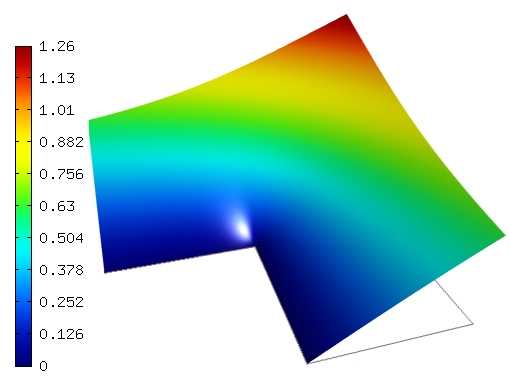
\includegraphics[height=5cm]{nist/nist-2/solution.png}
\caption{The solution to NIST-2 benchmark problem.}
\label{fig:sln-nist02}
\end{figure}

\begin{figure}[!ht]
\centering
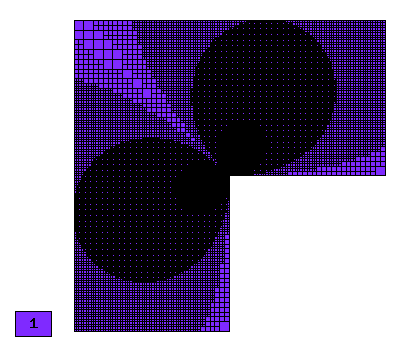
\includegraphics[height=3.7cm]{nist/nist-2/mesh_h1_aniso.png}
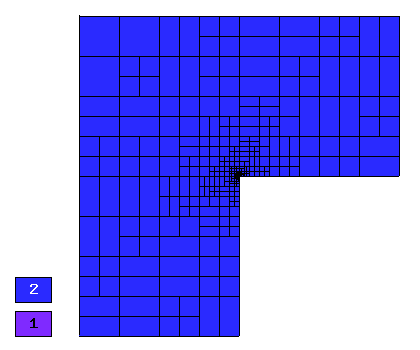
\includegraphics[height=3.7cm]{nist/nist-2/mesh_h2_aniso.png}
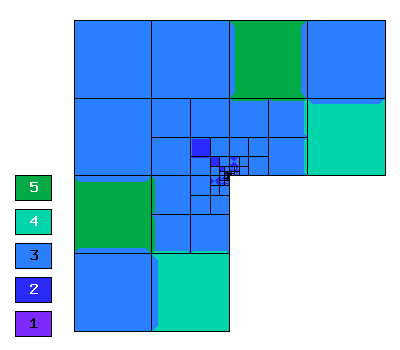
\includegraphics[height=3.7cm]{nist/nist-2/mesh_hp_aniso.png}
\caption{
Final mesh (left) with 46097 DOF and the resulting
relative error estimate in $H^1$-norm of 1.30193e-01 \% for $h$-FEM with linear elements.
Final mesh (middle) with 1289 DOF and the resulting
relative error estimate in $H^1$-norm of 8.26847e-02 \% for $h$-FEM with quadratic elements.
Final mesh (right) with 622 DOF and the resulting 
relative error estimate in $H^1$-norm of 8.15289e-02 \% for $hp$-FEM with anisotropic refinements.}
\label{fig:nist-2-hp-aniso}
\end{figure}

%\begin{figure}[!ht]
%\centering
%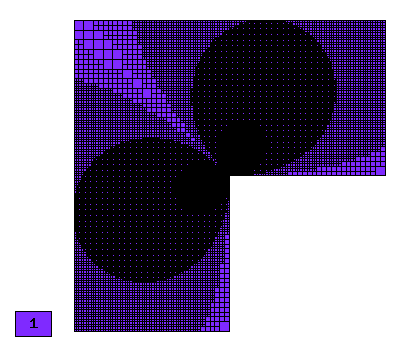
\includegraphics[height=5cm]{nist/nist-2/mesh_h1_aniso.png}\ \
%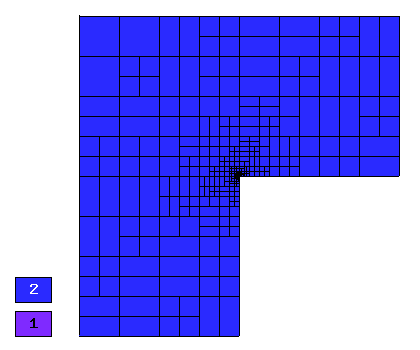
\includegraphics[height=5cm]{nist/nist-2/mesh_h2_aniso.png}
%\caption{Final mesh for $h$-FEM with linear and quadratic elements.}
%\label{fig:nist-2-h-aniso}
%\end{figure}

Figs. \ref{fig:nist-2-conv} compare all
three approaches to automatic adaptivity from the point
of view of DOF and CPU convergence.

\begin{figure}[!ht]
\centering
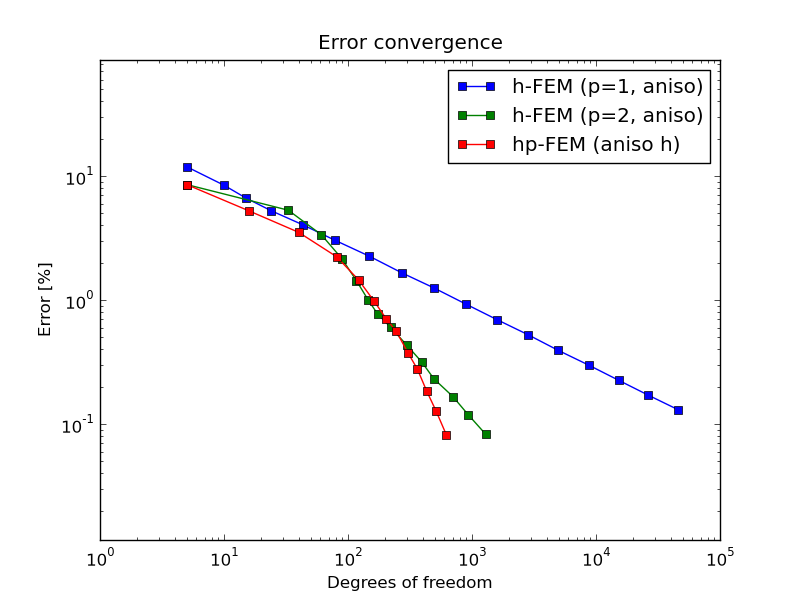
\includegraphics[height=5cm]{nist/nist-2/conv_dof_aniso.png}\ \
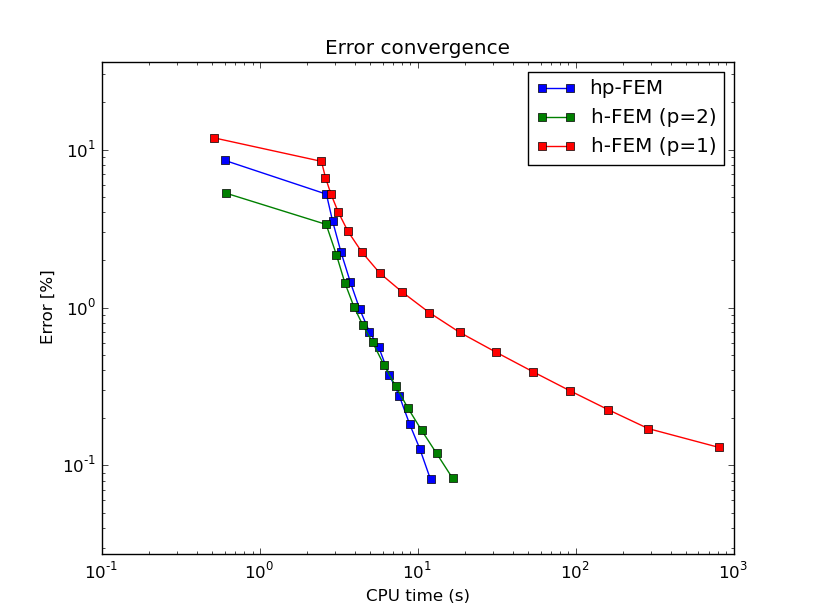
\includegraphics[height=5cm]{nist/nist-2/conv_cpu_aniso.png}
\caption{DOF and CPU time convergence graphs.}
\label{fig:nist-2-conv}
\end{figure}

